%
\section{System architecture}
\label{sec:system-architecture}
In this section, the system architecture is devised in the \gls{hw} and \gls{sw} components, using the system overview as a starting point. 

\subsection{Hardware architecture}
\label{sec:hardw-arch}
%
The diagram in Fig.\ref{fig:hw-arch} represents an initial hardware big picture in order to facilitate the objective identification.
As it can bee seen, the diagram is divided in four distinguished parts: \emph{External Environment}, \emph{Local System}, \emph{Remote Server} and \emph{Remote Client}.

Firstly, the \texttt{External Environment} represents all the environment that interacts with the system. In this case, these are all its users - normal users, brands and staff.

Secondly, the \texttt{Local System} is composed for the main controller, which is the Raspberry Pi 4B. 
This \gls{soc} is responsible to control all the Local System and to establish connection with the remote server through its included WiFi module. 
The board is powered connecting it to the electrical network. 
Then, it has several blocks connected to it:
%
\begin{item-c}
\item \emph{Motion Detection}: used to detect the users and switch from normal mode to interaction mode;
\item \emph{Fragrance Diffusion Actuator}: used to diffuse the fragrance onto the air;
\item \emph{Camera}: used to capture image that is then processed;
\item \emph{Speakers}: used to produce advertisements sounds;
\item \emph{Screen}: used to produce video clips of advertisements.
\end{item-c}
%

In third place, the \texttt{Remote Server} has a server node running in another machine that can be one computer or a main frame.
The remote server establishes connection with the cloud that has stored all the data from all databases.

Lastly, the \texttt{Remote Client} which can be a computer, a tablet or a smart phone to run the \gls{mdo} management application.
%
\begin{figure}[htb!]
\centering
    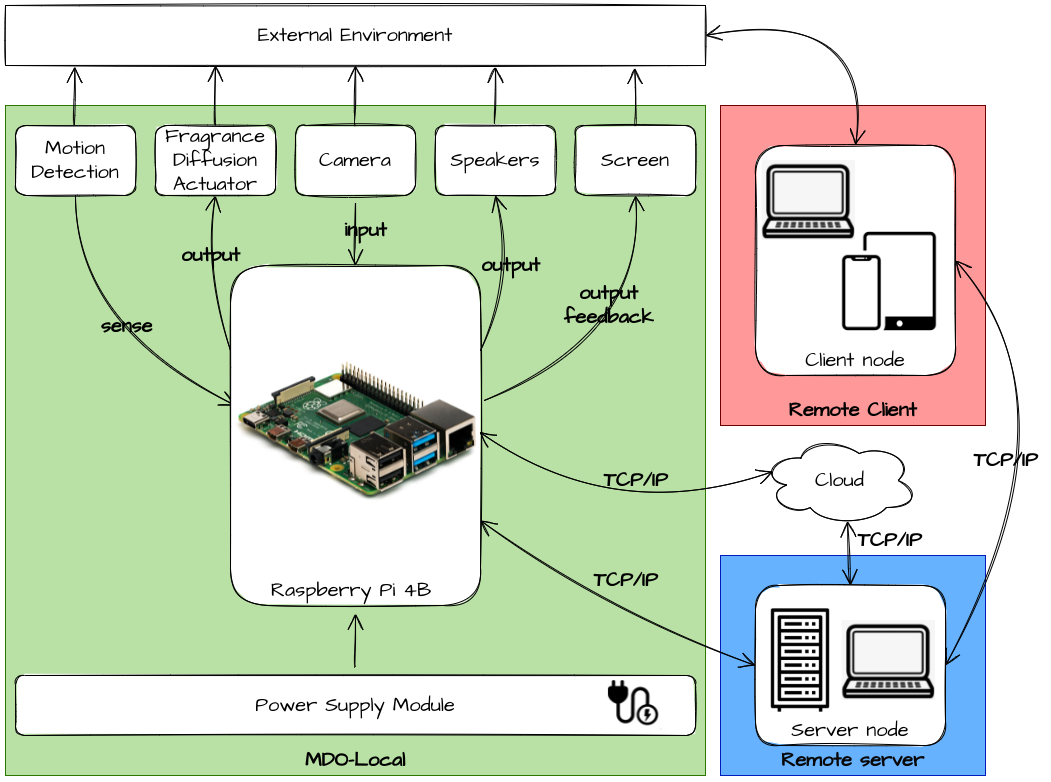
\includegraphics[width=0.8\columnwidth]{./img/HW_Architecture.png}
  \caption{\gls{hw} architecture diagram}%
\label{fig:hw-arch}
\end{figure}
%
%
\subsection{Software architecture}
\label{sec:softw-arch}
In this section the \gls{sw} architecture for \gls{mdo-rc}, \gls{mdo-rs}, and
\gls{mdo-l} subsystems is presented, defining its \gls{sw} stack.

\subsubsection{MDO remote client}
\label{sec:mdo-remote-client}
%
Fig.~\ref{fig:sw-arch-rc} illustrates the \gls{sw} architecture for the remote
client, representing its \gls{sw} stack.
It is comprised of the following layers:
\begin{item-c}
\item \emph{Application}: contains the remote client application. The
  \texttt{Brand} and \texttt{Admin} members interact with the \gls{ui}, which is
  the visual part of the interface. The \texttt{\gls{ui} engine} is notified and
  handles all \gls{ui} events --- internal or external --- providing the \texttt{UI}
  with feedback for its users. The relevant commands
  are then parsed --- \texttt{Parser} component --- and responded. The commands
  are then translated to the appropriate \gls{db} queries and responded through
  the \texttt{DB Manager}. The \texttt{Comm Manager} is responsible for
  encapsulating the \gls{db} queries into the respective \gls{tcp-ip} frames to
  be sent to the \texttt{Remote Server} as well as unwrap the incoming server
  responses.
\item \emph{Middleware}: contains the \gls{tcp-ip} framework supporting these
  communication protocols as part of \gls{osi} model for internet
  applications. It manages the incoming/outgoing \gls{tcp-ip} frames by
  providing the adequate protocol handshaking and queueing and timing aspects of
  the bytes to send/receive.
\item \emph{OS \& BSP} --- \gls{os} \& \gls{bsp}: it contains the low-level and
  communication drivers required to handle input (keyboard/touch), output
  (screen) and communication to the \texttt{Remote Server}.
\end{item-c}
It should be noted that for desktop and mobile applications, the
\texttt{Middleware} and \texttt{OS \& BSP} layers are usually abstracted by the
\gls{os}, thus, the relevant \gls{api}s should be used.
%
\begin{figure}[htb!]
\centering
    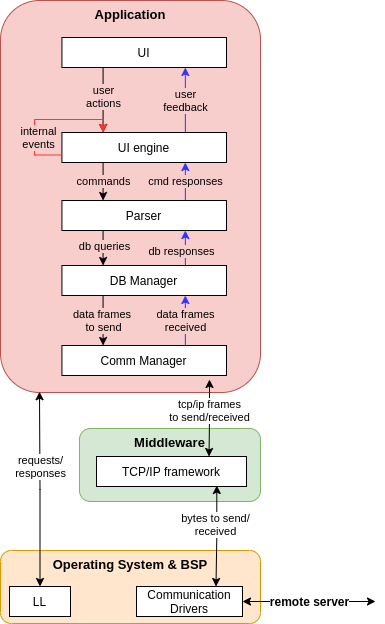
\includegraphics[width=0.55\columnwidth]{./img/sw-arch-rc.png}
  \caption{\gls{sw} architecture diagram: remote client}%
\label{fig:sw-arch-rc}
\end{figure}

\subsubsection{MDO remote server}
\label{sec:mdo-remote-server-1}
%
Fig.~\ref{fig:sw-arch-rs} illustrates the \gls{sw} stack for architecture for
the remote server.
It is comprised of the following layers:
\begin{item-c}
\item \emph{Application}: contains the remote server application. It provides a
  \gls{cli} to handle \texttt{Remote client} requests.  The \gls{cli} engine
  is notified and handles all \gls{ui} events --- internal or external ---
  providing the appropriate feedback. The relevant commands
  are then parsed --- \texttt{Parser} component --- and responded: \gls{db}
  queries are handled by the \texttt{\gls{rdbms}} issuing \gls{db} transactions;
  other commands received from the \texttt{Remote Client} are handled internally
  and translated, being dispatched to the \texttt{Local
    System} by the \texttt{Comm Manager}  (via \texttt{Communication drivers}). Internal events can also
  trigger the \texttt{\gls{rdbms}} to issue database transactions for the
  \texttt{Remote Client} or \texttt{Local System}.
  The \texttt{Comm Manager} is responsible for wrapping\slash unwrapping the data
  frames received by or sent to the \texttt{Remote Client} or \texttt{Local System}.
\item \emph{Middleware}: contains the \gls{rdbms} framework supporting the
  management of the relational databases using database transactions.
\item \emph{OS \& BSP} --- \gls{os} \& \gls{bsp}: it contains the \texttt{Communication}
  drivers to the handle requests from the \texttt{Remote Client}, and the
  \texttt{File I/O} drivers to manipulate \gls{db} transactions from\slash to storage.
\end{item-c}
%
\begin{figure}[htb!]
\centering
    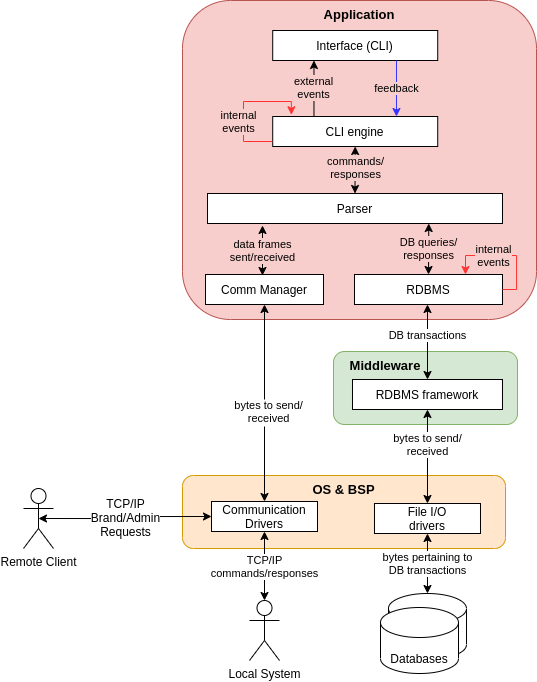
\includegraphics[width=0.55\columnwidth]{./img/sw-arch-rs.png}
  \caption{\gls{sw} architecture diagram: remote server}%
\label{fig:sw-arch-rs}
\end{figure}
%
It should be noted that the \texttt{Remote Server} main functions are:
\begin{item-c}
\item provide relational databases for easier management of all entities and
  respective data in the system;
\item decompose the relationship many-to-many, between the remote clients and
  local systems --- many remote clients may want to connect to different local
  systems; 
\item decouple the architecture as the \texttt{Remote Client} should not know
the \gls{ip} address of every local system it may potentially try to access,
acting as a proxy server.
\end{item-c}
%
\subsubsection{MDO local system}
\label{sec:mdo-local-system-1}
%
Fig.~\ref{fig:sw-arch-local} illustrates the \gls{sw} stack for architecture for
the \texttt{Local System}.
It is comprised of the following layers:
\begin{item-c}
\item \emph{Application}: contains the local system application. It provides a
  \gls{ui} to handle \texttt{User} interaction.  The \texttt{Interface} engine
  is notified and handles all \gls{ui} events --- internal or external ---
  through gesture recognition, providing the appropriate feedback. The relevant
  commands are then parsed --- \texttt{Supervisor} component --- and responded: \gls{db}
  queries are handled by the \texttt{Database manager} issuing \gls{db}
  transactions for internal databases;
  commands received from the \texttt{Remote Server} to monitor or control the
  system are handled internally
  and responded back by the \texttt{Comm Manager}  (via \texttt{Communication
    drivers}); mode management is performed.
  Internal events can also trigger the \texttt{Database manager} to issue
  database transactions to update the \texttt{Local System}.
  The \texttt{Comm Manager} is responsible for wrapping\slash unwrapping the data
  frames received by or sent to the \texttt{Remote Server}.
\item \emph{Middleware}: contains: the \gls{db} framework supporting the
  management of the internal databases using database transactions; the \gls{cv}
  framework that handles gesture and facial recognition; image filtering and
  \gls{gif} frameworks for multimedia; social media framework.
\item \emph{OS \& BSP} --- \gls{os} \& \gls{bsp}: contains: the \texttt{Communication}
  drivers to the handle requests from the \texttt{Remote Server} and for social
  media sharing, and, potentially the \gls{api} calls to cloud-based image
  filtering frameworks, depending on the application profiling; the
  \texttt{File I/O} drivers to manipulate internal \gls{db} transactions
  from\slash to storage; audio, video and fragrance diffuser actuator drivers
  for normal mode; the camera driver for camera feed; the detection sensor
  driver to signal a \texttt{User} is in range, triggering the switch from
  normal mode to interaction mode.
\end{item-c}
%
\begin{figure}[htb!]
\centering
    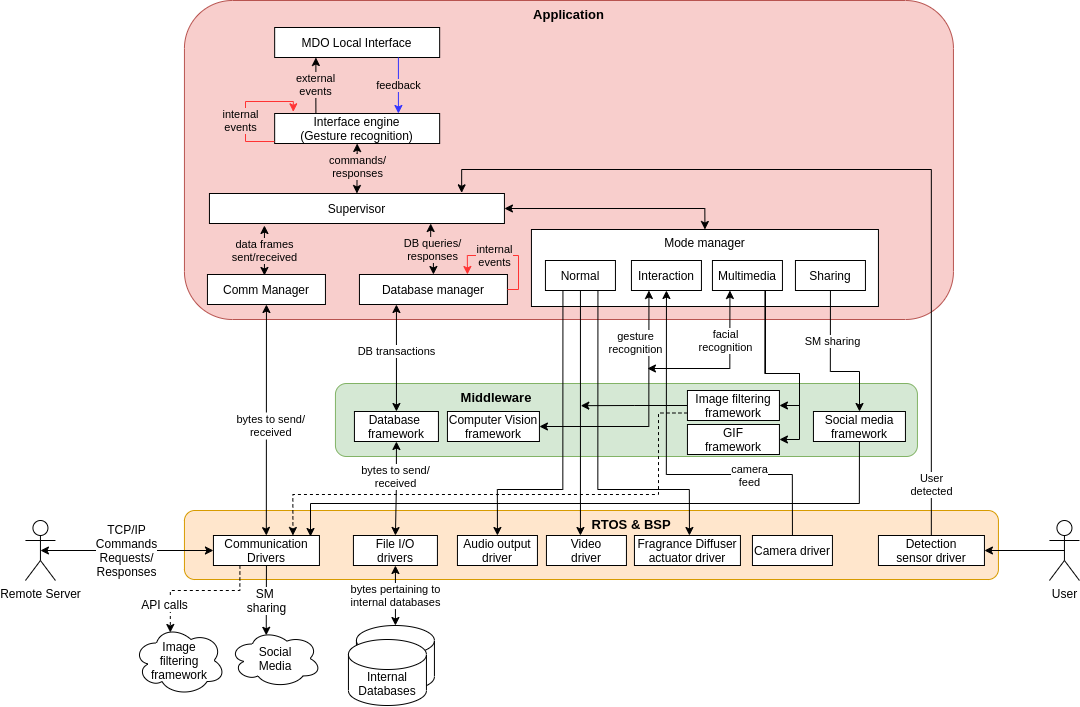
\includegraphics[width=1.0\columnwidth]{./img/sw-arch-local.png}
  \caption{\gls{sw} architecture diagram: local system}%
\label{fig:sw-arch-local}
\end{figure}
%
%
%%% Local Variables:
%%% mode: latex
%%% TeX-master: "../../../dissertation"
%%% End:
